The previous chapters built the filtering methods in general form, the Kalman filter for linear Gaussian state space models and the extended Kalman filter for non-linear ones. In this chapter we use them on real financial data, with the goal of applying the models to stock price series. The task is to predict the next value of a price series one step ahead, and every model is fitted and tested on the same series, so that the results can be compared directly.

We look at two families of models. The mean models let the average return change over time, which stays within reach of the Kalman filter. The variance models let the size of the returns change over time, which is non-linear and needs the extended Kalman filter. The independent and identically distributed (i.i.d.) model is the baseline for both. We begin by putting the data into a form these models can use. 


\section{Prices and returns}\label{sec:prices-returns}
Let $p_t$ denote the price of the asset at the discrete time index $t$. Rather than model the price directly, we work with its logarithm, from which this section builds the two quantities the models of this chapter observe, the log-price and the log-return. There are two reasons for taking logarithms. First, prices are always positive and often span a wide range over a long sample, so a model with additive Gaussian noise on $p_t$ fits the data poorly and can even place probability on negative prices. Second, on the log scale a multiplicative change becomes an additive one, which is the form the additive-noise state space models of this chapter need.

The first quantity is the log-price 
\begin{equation}\label{eq:logprice}
  s_t \;=\; \log p_t ,
\end{equation}
which measures the price on a scale where equal percentage moves have equal size. Its advantage is that it still says where the price stands, so a model for $s_t$ predicts the next price directly, and additive noise on this scale keeps the implied price positive. Its drawback is that it inherits the trend of the price, so its typical value in one part of the sample says little about its typical value in another.

The second quantity is the log-return\footnote{In this chapter $r_t$ denotes the return, following standard usage in finance. It is not the measurement noise of the filtering chapters, which we write as $\varepsilon_t$ throughout this chapter.}
\begin{equation}\label{eq:logreturn}
  r_t \;=\; s_t - s_{t-1} \;=\; \log \frac{p_t}{p_{t-1}} .
\end{equation}

the first difference of the log-price. For the small changes typical of financial data it is close to the ordinary relative return $(p_t - p_{t-1})/p_{t-1}$, so we can read $r_t$ as the fractional gain or loss over one step. Its advantage is stability over time. A series whose mean and variance do not change is called stationary, and returns come much closer to this than prices do, so parameters estimated on one stretch of the data remain meaningful on the next~\cite[Ch.~2]{palomar:portfolio_optimization}. This is what makes it sensible to fit a model on past data and then ask it to predict. Its drawback is that the level is gone, since a return says how much the price moved and not where it stands, so the price has to be rebuilt as $s_t = s_{t-1} + r_t$ whenever we want to see it. How far the stability of returns actually reaches is a question we return to when we model the variance.

Which of the two a model uses depends on what its hidden state describes. The level models of Section~\ref{sec:mean-modeling} take the log-price as their observation, because their state is the underlying level of the series, while the i.i.d.\ model, the autoregressive models and the stochastic volatility model take the log-return, because they describe how the series moves rather than where it stands. Both scales carry the same one-step prediction error, so the choice does not affect the comparison in Section~\ref{sec:model-comparison}. 

\section{The modeling framework}\label{sec:framework}

\subsection{The state space form of the models}
Every model in this chapter is a state space model in the sense of Chapter~\ref{chap:basic}, and we write each of them below in the same two-line scheme, one line for the transition and one for the measurement, with transition matrix $\mathbf{A}$ and observation matrix $\mathbf{H}$ as in Chapter~\ref{chap:kalman}. Only the stochastic volatility model at the end of the chapter has a measurement that is a non-linear function of the state.

\subsection{Training, testing and scoring}
Every model is treated in the same two steps. First we estimate its unknown parameters, collected in a vector $\boldsymbol{\theta}$, which are the noise variances and later the autoregressive coefficients. As the filter runs it predicts each observation one step ahead, and the sizes of these prediction errors say how well a given $\boldsymbol{\theta}$ explains the data. Chapter~\ref{chap:parameter} collects them into the energy function, the negative log-likelihood, so minimizing it over $\boldsymbol{\theta}$ is maximum likelihood estimation~\cite[Ch.~12]{sarkka:bayesian_filtering}. Second, with $\boldsymbol{\theta}$ fixed, we run the filter over the data.

We keep these two roles apart on the data as well. The series is split into a training part, the first $80\%$ of the sample, on which the parameters are estimated, and a test part, the last $20\%$, which the fitting never sees. There the parameters stay frozen, and at every step we record the one-step-ahead forecast made before that value is observed. It is these forecasts that are scored in Section~\ref{sec:model-comparison}.

\subsection{How the models are computed}
The pipeline itself is written in Python. The matrix algebra uses \texttt{numpy} \cite{numpy}, the data handling \texttt{pandas} \cite{pandas}, and the minimization of the energy function the Nelder-Mead simplex method from \texttt{scipy.optimize} \cite{scipy}, which is the gradient-free option described in Chapter~\ref{chap:parameter}. The filters themselves are not taken from a library. They are implemented directly from the recursions of Chapter~\ref{chap:kalman} and Chapter~\ref{chap:nonlinear}, which keeps the code close to the equations of this thesis and makes every step visible.

For a given model the pipeline runs in five steps.

\begin{enumerate}
  \item Build the state space matrices $\mathbf{A}, \mathbf{H}, \mathbf{Q}, R$ from the parameter vector $\boldsymbol{\theta}$.
  \item Run the filter over the training data and accumulate the energy function.
  \item Minimize the energy over $\boldsymbol{\theta}$ to obtain the parameter estimates.
  \item Run the filter over the test data with $\boldsymbol{\theta}$ frozen, recording the one-step-ahead forecast at every step.
  \item Score those forecasts with the mean squared error of Section~\ref{sec:model-comparison}.
\end{enumerate}

The first step is the only one that differs between models. For the autoregressive model of Section~\ref{sec:mean-modeling} it builds the companion form of \eqref{eq:ar1-ss} from the coefficients and the innovation variance.

\begin{minted}{python}
def ar_to_ssm(phi, sigma2):
    p = len(phi) - 1              # AR order, phi = [phi_0, ..., phi_p]
    d = p + 1                     # state = (1, r_t, ..., r_{t-p+1})
    A = np.zeros((d, d))
    A[0, 0] = 1.0                 # keep the constant component
    A[1, :] = phi                 # the autoregressive row
    for i in range(2, d):
        A[i, i - 1] = 1.0         # shift the older lags down
    H = np.zeros((1, d)); H[0, 1] = 1.0
    Q = np.zeros((d, d)); Q[1, 1] = sigma2
    R = np.array([[0.0]])         # no measurement noise
    return A, H, Q, R
\end{minted}

The second step is the same for every linear model of this chapter. It is the Kalman filter recursion of Theorem~\ref{thm: kalman filter}, with the energy function of Chapter~\ref{chap:parameter} accumulated as the filter goes.

\begin{minted}{python}
for t in range(T):
    x = A @ x                                # prediction
    P = A @ P @ A.T + Q
    y_pred[t] = (H @ x).item()               # one-step-ahead forecast

    v = y[t] - y_pred[t]                     # innovation
    S = (H @ P @ H.T + R).item()             # innovation covariance
    K = (P @ H.T) / S                        # Kalman gain
    x = x + K.flatten() * v                  # update
    P = P - K @ (H @ P)

    energy += 0.5 * (np.log(2 * np.pi * S) + v * v / S)
\end{minted}

For the stochastic volatility model of Section~\ref{sec:variance-modeling} the same loop is used, with the linearized measurement of the extended Kalman filter in place of $\mathbf{H}$.

With this framework fixed, we can build the models one at a time, starting from the one that assumes the least.

\section{The i.i.d.\ model}\label{sec:iid}

We start with the simplest possible model, one that ignores time completely. It assumes that the log-returns are independent and identically distributed,
\begin{equation}\label{eq:iid}
  r_t \;=\; \mu + \varepsilon_t , \qquad
  \varepsilon_t \overset{\text{i.i.d.}}{\sim} \mathcal{N}(0, \sigma^2).
\end{equation}
Identically distributed means that every return is drawn from the same distribution, here a Gaussian with a fixed mean $\mu$ and a fixed variance $\sigma^2$. Independent means that a return carries no information about the next one. Together these two assumptions strip the series of any memory. The distribution of the next return is the same no matter what has happened before, so the best one-step-ahead prediction of the return is just the constant $\mu$, which we estimate by the sample mean of the training returns.

It helps to see what this assumption says about the price itself. Adding the returns back up, the log-price is
\begin{equation}\label{eq:rw-drift}
\begin{aligned}
  s_t &= s_{t-1} + r_t \\
      &= s_{t-1} + \mu + \varepsilon_t ,
\end{aligned}
\end{equation}
so at each step the log-price takes a fixed average step $\mu$ plus Gaussian noise. A process of this form, a random walk whose steps have a nonzero mean, is called a \emph{random walk with drift}, and $\mu$ is the drift. When the drift is zero the best forecast of tomorrow's log-price is simply today's. This is the statement of the efficient market hypothesis, according to which the current price already reflects all available information, so that no better forecast than the current price is possible \cite[Ch.~3]{palomar:portfolio_optimization}.

Figure~\ref{fig:iid-hist} shows the model fitted to the training returns. Returns at both extremes, large gains and large losses, occur more often than the fitted normal allows. Each bar of the histogram covers a small interval of return values, and its area is the share of trading days whose log-return falls into that interval. The histogram is normalized so that its total area is one, which makes it directly comparable to the red curve, the density of the fitted Gaussian $\mathcal{N}(\hat{\mu}, \hat{\sigma}^2)$ with the sample mean $\hat{\mu}$ and the sample variance $\hat{\sigma}^2$ of the training returns. If the i.i.d.\ model were exactly right, the bars would follow this curve.

They do so around the center, where the fit is reasonable, so a Gaussian is not an absurd description of a typical day. The mismatch sits at the peak and in the tails. The peak at the center is higher than the fitted density, so there are more very calm days than the Gaussian predicts. And a few isolated bars stand far out, near four standard deviations from the mean, where the fitted density is practically zero. In numbers, about $1\%$ of the training returns lie more than three standard deviations from the mean, roughly three times as many as the fitted normal allows. These heavy tails are one of the stylized facts of returns~\cite[Ch.~2]{palomar:portfolio_optimization}, and they point to a variance that changes over time. When calm and turbulent periods alternate, the pooled returns contain more extreme values than any single Gaussian allows.

\begin{figure}
  \centering
  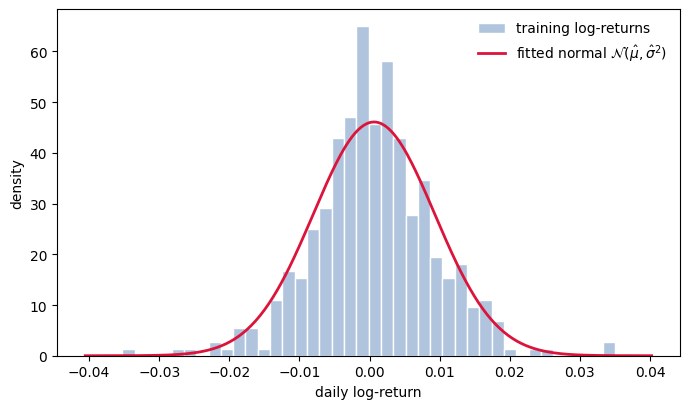
\includegraphics[width=0.7\linewidth]{Figures/iid_returns_hist.png}
  \caption{Histogram of the training log-returns of the gold series with the
  fitted normal density $\mathcal{N}(\hat{\mu},\hat{\sigma}^2)$. The center of
  the distribution is matched reasonably well, while the data show a sharper
  peak and heavier tails than the fitted Gaussian.}
  \label{fig:iid-hist}
\end{figure}

The i.i.d.\ model is our baseline, and every later model is measured against it. By fixing both the mean and the variance it treats every period of the market the same, which real return series do not. The next two sections relax these two assumptions in turn, first the mean and then the variance.

\section{Mean models}\label{sec:mean-modeling}
The first family of models lets the average return change over time. Under the efficient market hypothesis of Section~\ref{sec:iid} this should not help at all. A competing view holds that markets are not fully efficient and that returns carry some structure over time, so that the average return moves rather than staying at one fixed value~\cite[Section~4.1]{palomar:portfolio_optimization}. We do not settle this debate. We take the second view as a hypothesis and test it, replacing the single mean $\mu$ of the i.i.d.\ model by a hidden state that the filter tracks over time. On this data the answer will turn out to be that it helps very little.

This section does this in three ways. The variance is kept constant for the moment and becomes the subject of Section~\ref{sec:variance-modeling}. All three models here are linear Gaussian state space models, so the Kalman filter of Chapter~\ref{chap:kalman} applies without any change, and their parameters are estimated by the energy-based maximum likelihood described in Section~\ref{sec:framework}. We present them from the simplest to the most flexible, each one relaxing an assumption of the one before~\cite[Ch.~4]{palomar:portfolio_optimization}.

\subsection{The local level model}
\textbf{Observation:} the log-price $s_t$ of Section~\ref{sec:prices-returns}, so the model forecasts the next log-price.
The smallest step beyond the i.i.d.\ model is to let the mean itself change over time. We introduce a hidden state $x_t$ called the \emph{level} of the series, the smooth underlying log-price we would see if there were no noise, so that the observation $y_t$ is the level plus measurement noise. It plays the same role for the price that the true position played for the tracked drone in Chapter~\ref{chap:kalman}, a smooth path hidden behind jagged data, and we call it \emph{latent} because we never observe it directly. 

Instead of holding the level fixed, as the i.i.d.\ model holds $\mu$, we let it follow a random walk, so it can drift from one step to the next. The model is
\begin{equation}\label{eq:rw}
\begin{aligned}
  \text{transition:}\quad & x_t = x_{t-1} + q_{t-1}, && q_{t-1} \sim \mathcal{N}(0, Q), \\
  \text{measurement:}\quad & y_t = x_t + \varepsilon_t, && \varepsilon_t \sim \mathcal{N}(0, R),
\end{aligned}
\end{equation}
with transition matrix $\mathbf{A}=1$ and observation matrix $\mathbf{H}=1$. This is the \emph{local level model}, also called the random walk model, since the level moves as a random walk and all its movement comes from the process noise $q_{t-1}$. The two variances play opposite roles. A large $Q$ lets the level move quickly and makes the filter follow the data closely, while a large $R$ treats the observations as noisy and makes the filter smooth over them. Specializing the Kalman prediction step to \eqref{eq:rw} gives
\begin{equation}\label{eq:rw-pred}
  x_{t+1\mid t} = x_{t\mid t},
  \qquad
  P_{t+1\mid t} = P_t + Q,
\end{equation}
so the one-step-ahead forecast of the level is the current filtered estimate. Unlike the constant i.i.d.\ forecast, this estimate is updated at every step, so the forecast moves with the data.

Figure~\ref{fig:rw-gold} shows the model on the test segment. The prediction is the observed series shifted by one step. Three curves are drawn over the time index of the test segment, the observed data, the filtered level and the dashed one-step-ahead prediction, all shown on the price scale, since the model runs on the log-price and is transformed back for the plot. Fitting \eqref{eq:rw} to the gold series gives a very small measurement variance $R$, so the filter trusts the observations almost completely and the filtered level lies on top of them.

\begin{figure}
  \centering
  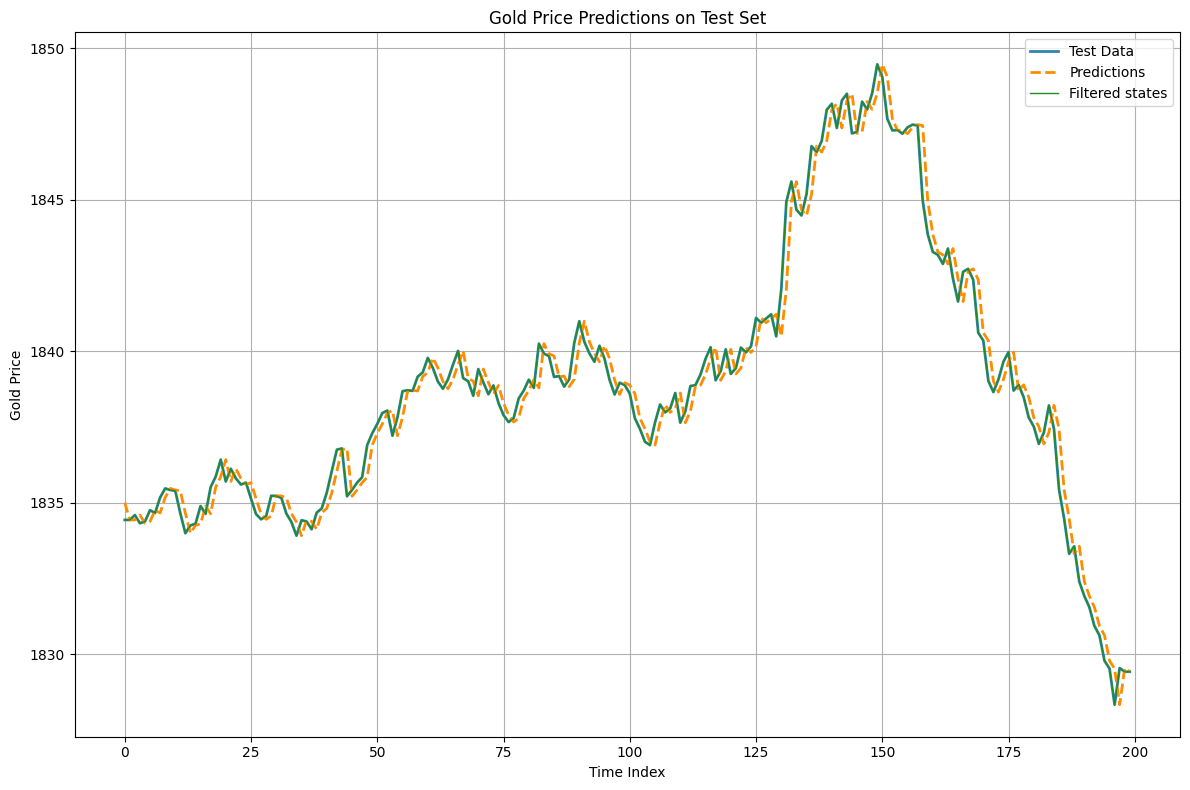
\includegraphics[width=0.7\linewidth]{Figures/Gold Price Predictions Random Walk.png}
  \caption{One-step-ahead predictions of the gold price under the local level
  model. The filtered level tracks the data closely, while the prediction is
  the previous filtered level.}\label{fig:rw-gold}
\end{figure}
On its own the local level model therefore adds little to the i.i.d.\ forecast.

\subsection{The local linear trend model}
\textbf{Observation:} the log-price $s_t$, so the model forecasts the next log-price.
The local level model expects the next level to equal the current one, even when the series has been climbing or falling steadily. The local linear trend model extends it by a second state component, a slope that carries the current direction of movement forward~\cite[Section~4.1]{triantafyllopoulos:bayesian_state_space}. Because the level is the log-price, its rate of change is the expected one-step return, so the slope is a drift that is now allowed to vary over time, unlike the constant drift $\mu$ of the i.i.d.\ model. The state is $\mathbf{x}_t = (\ell_t, b_t)^\top$, with local level $\ell_t$ and local slope $b_t$, and the model is

\begin{equation}\label{eq:llt-state}
  \text{transition:}\quad
  \mathbf{x}_t =
  \underbrace{\begin{bmatrix} 1 & 1 \\ 0 & 1 \end{bmatrix}}_{\mathbf{A}}
  \mathbf{x}_{t-1} + \mathbf{q}_{t-1},
  \qquad
  \mathbf{q}_{t-1} \sim \mathcal{N}\!\left(\mathbf{0},\,
  \mathbf{Q}\right),
  \quad
  \mathbf{Q} = \begin{bmatrix} \sigma_\ell^2 & 0 \\ 0 & \sigma_b^2 \end{bmatrix},
\end{equation}
\begin{equation}\label{eq:llt-obs}
  \text{measurement:}\quad
  y_t = \underbrace{\begin{bmatrix} 1 & 0 \end{bmatrix}}_{\mathbf{H}}\mathbf{x}_t + \varepsilon_t,
  \qquad
  \varepsilon_t \sim \mathcal{N}(0, R).
\end{equation}
The slope enters the level at every step, and that is the whole difference to the local level model. Written out component by component, the dynamics read

\begin{equation}\label{eq:llt-components}
  \ell_t = \ell_{t-1} + b_{t-1} + \eta_t,\qquad
  b_t   = b_{t-1} + \zeta_t,  
\end{equation}

with level noise $\eta_t \sim \mathcal{N}(0,\sigma_\ell^2)$ and slope noise $\zeta_t \sim \mathcal{N}(0,\sigma_b^2)$. The first equation moves the level by the current slope before adding noise, and the second lets the slope itself drift as a random walk. Setting the slope to zero returns the local level model of \eqref{eq:rw}, so the trend model contains it as a special case. The Kalman prediction step now propagates both components,

\begin{equation}\label{eq:llt-pred}
  \mathbf{x}_{t+1\mid t} = \mathbf{A}\,\mathbf{x}_{t|t},
  \qquad
  \mathbf{P}_{t+1\mid t} = \mathbf{A}\,\mathbf{P}_t\,\mathbf{A}^\top + \mathbf{Q},
\end{equation}

so the predicted level is the current level carried forward along the current slope, $\hat{\ell}_{t+1\mid t} = \hat{\ell}_t + \hat{b}_t$. This lets the model keep up with a sustained drift that the plain random walk would always lag behind.  Figure~\ref{fig:llt-gold} shows the fit on a short stretch of the gold test segment, with axes and curves as in Figure~\ref{fig:rw-gold}. The prediction now extrapolates along the estimated slope instead of repeating the last level. Where the series keeps its direction this reduces the one-step lag, and at sharp turns the extrapolation overshoots briefly before the slope estimate adjusts.

\begin{figure}
  \centering
  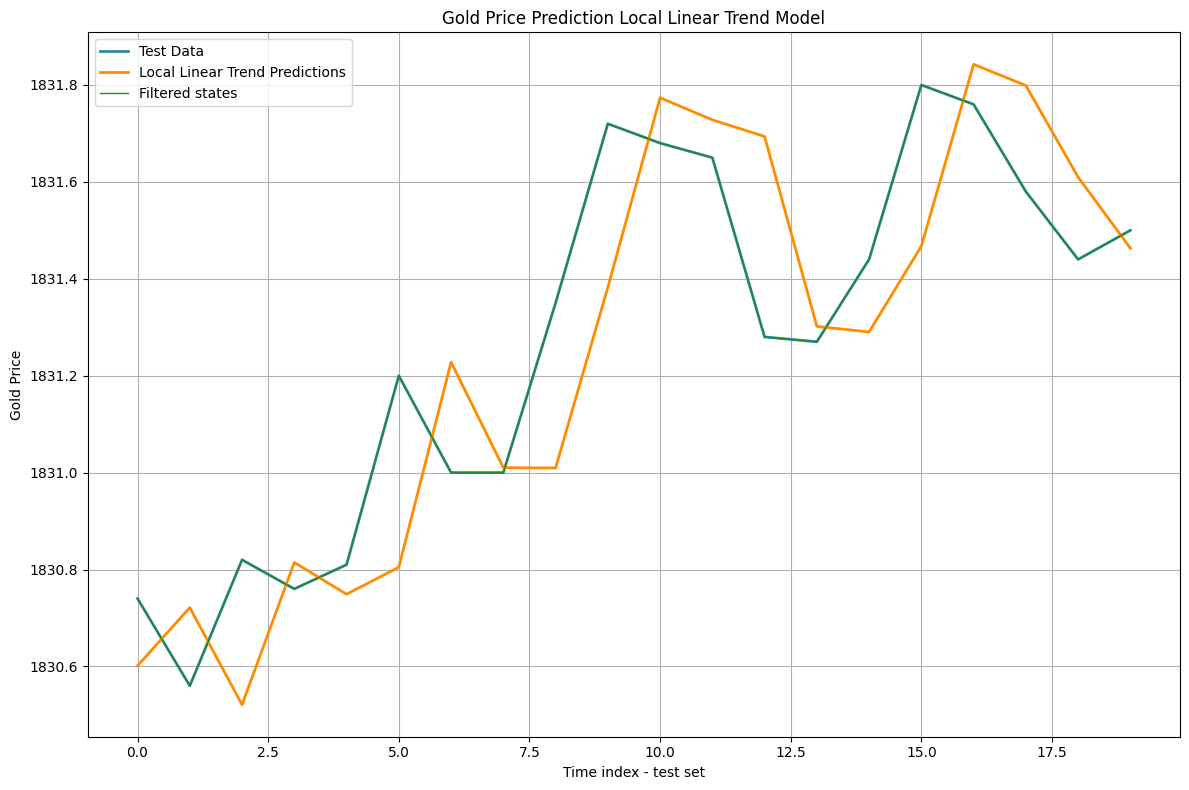
\includegraphics[width=0.7\linewidth]{Figures/Gold Price Predictions Local Linear Trend Model.png}
  \caption{One-step-ahead predictions of the gold price under the local linear
  trend model. The estimated slope lets the prediction extrapolate the local
  direction of the series.}\label{fig:llt-gold}
\end{figure}

The slope gives the model a sense of direction, but it still describes only the level of the series. The last model of this section takes the opposite route and works directly with the returns.

\subsection{Autoregressive models}
\textbf{Observation:} the log-return $r_t$, so the model forecasts the next return directly.
The local level and local linear trend models both act on the level of the series. An autoregressive model instead writes the current value as a weighted sum of its own recent past, which is the standard way to capture short-range dependence in a return series
\cite[Section~7.2]{triantafyllopoulos:bayesian_state_space}.  Depending on the sign of the coefficients this can express momentum, where a move tends to continue, or mean reversion, where a move tends to be undone. The autoregressive model of order $p$ is
\begin{equation}\label{eq:arp}
  r_t = \varphi_0 + \sum_{i=1}^{p} \varphi_i\, r_{t-i} + \epsilon_t,
  \qquad \epsilon_t \sim \mathcal{N}(0,\sigma^2),
\end{equation}
with intercept $\varphi_0$ and coefficients $\varphi_1,\dots,\varphi_p$. An autoregressive model of order $p$ does not fit the filter directly, because the Kalman filter needs a state that depends only on the step before, while $r_t$ in \eqref{eq:arp} depends on the $p$ preceding values. We obtain a first-order state by stacking the last $p$ values into the state vector. Keeping the intercept as a constant component, the order-one case has state $\mathbf{x}_t = (1, r_t)^\top$ and
\begin{equation}\label{eq:ar1-ss}
\begin{aligned}
  \text{transition:}\quad & \mathbf{x}_t =
  \underbrace{\begin{bmatrix} 1 & 0 \\ \varphi_0 & \varphi_1 \end{bmatrix}}_{\mathbf{A}}
  \mathbf{x}_{t-1} + \begin{pmatrix} 0 \\ \epsilon_t \end{pmatrix}, \\
  \text{measurement:}\quad & y_t =
  \underbrace{\begin{bmatrix} 0 & 1 \end{bmatrix}}_{\mathbf{H}} \mathbf{x}_t
  + \varepsilon_t,
\end{aligned}
\end{equation}
where the process noise enters only the second component and is the autoregressive noise $\epsilon_t$ itself, with no measurement noise, $R = 0$, so the observation is the return exactly. For general $p$ the state collects the $p$ most recent values together with the constant, and $\mathbf{A}$ takes the companion form whose first row holds the coefficients $\varphi_0,\dots,\varphi_p$ and whose subdiagonal of ones shifts the remaining entries down by one at each step. The prediction step is again $\mathbf{x}_{t+1\mid t} = \mathbf{A}\,\mathbf{x}_{t|t}$, which reproduces the autoregressive recursion on the expected value.  

Figure~\ref{fig:ar-forecast} shows the fitted AR(2) model at work on the test segment, data the fit has never seen. The upper panel compares the realized gold price with its one-step-ahead forecast. At each test day the model predicts the next return from the two most recent returns, and the forecast price is the current price moved by this predicted return. The two curves are nearly indistinguishable, and the dashed forecast follows the solid realized price with a delay of one day, most visible at sharp turns. This is what a weak forecast looks like on the level of the price. Almost all of the forecast is simply the current price, and the model adds a small correction on top.

\begin{figure}
  \centering
  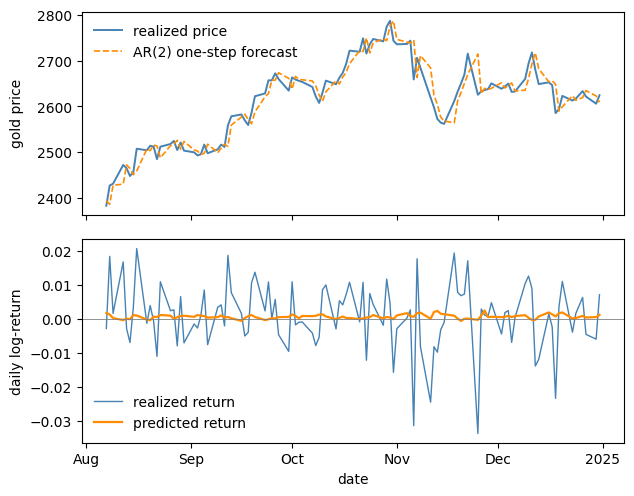
\includegraphics[width=0.8\linewidth]{Figures/ar_forecast_test.png}
  \caption{One-step-ahead AR(2) forecast on the test segment of the gold
  series. Top: realized price and forecast price, which is the previous price
  moved by the predicted return. Bottom: realized and predicted daily
  log-returns on the same scale. The predictable part of the daily move is an
  order of magnitude smaller than the move itself.}\label{fig:ar-forecast}
\end{figure}
With the mean now made time-varying in three ways, the variance has stayed fixed throughout. The next section turns to the variance and lets it follow a hidden process of its own.

\section{Variance models}\label{sec:variance-modeling}
We now turn to the variance, the typical size of the returns. Here the evidence is clearer than for the mean, and the filter does recover a hidden volatility from the data. Large moves tend to arrive in groups, a pattern called volatility clustering~\cite[Ch.~2]{palomar:portfolio_optimization}, and neither the fixed $\sigma^2$ of the i.i.d.\ model nor the fixed noise variances of the mean models can capture it. A stochastic volatility model makes the variance itself a hidden state with its own dynamics, so that calm and turbulent periods come out of the model instead of being assumed away~\cite[Section~7.3]{triantafyllopoulos:bayesian_state_space}.

Figure~\ref{fig:vol-clustering} shows this pattern in the training returns. Calm and turbulent phases alternate and last for weeks. The upper panel plots the daily log-returns over time, and the swings around zero are not equally large everywhere. The lower panel condenses this into one number per day, the standard deviation of the returns over the previous $20$ trading days, a simple local estimate of the current volatility. Under the i.i.d.\ model this curve should fluctuate closely around the single $\sigma$ of \eqref{eq:iid}. Instead it moves between about $0.004$ and $0.014$, so the typical daily move in the most turbulent phase is more than three times the one in the calmest phase, and it moves slowly enough that the current level of volatility carries information about tomorrow's. This persistence is what the stochastic volatility model below formalizes with a hidden state.

\begin{figure}
  \centering
  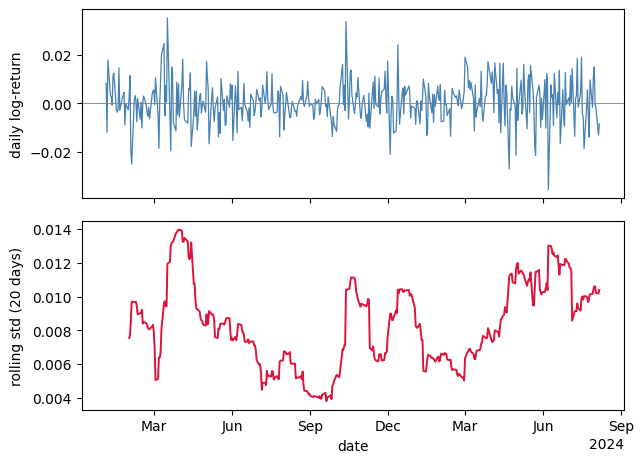
\includegraphics[width=0.8\linewidth]{Figures/vol_clustering.png}
  \caption{Volatility clustering in the training log-returns of the gold
  series. Top: daily log-returns. Bottom: rolling standard deviation over the
  previous $20$ trading days. Calm and turbulent phases alternate and persist
  for weeks.}
  \label{fig:vol-clustering}
\end{figure}

\subsection{The stochastic volatility model}
\textbf{Observation:} the demeaned log-return $r_t$, and after the transformation below its square $z_t = r_t^2$, so the model forecasts the size of the next return rather than its direction.
Let $r_t$ denote the demeaned log-return, that is, the return with its average already subtracted, so we can focus on its size alone. The model describes the changing variance through a hidden log-variance $h_t$ that follows a first-order autoregression,
\begin{equation}\label{eq:sv-state}
  \text{transition:}\quad
  h_t = \mu + \varphi\,(h_{t-1}-\mu) + \eta_t,
  \qquad \eta_t \sim \mathcal{N}(0,\sigma_\eta^2),
\end{equation}
and the return is this volatility times standard Gaussian noise,
\begin{equation}\label{eq:sv-obs}
  \text{measurement:}\quad
  r_t = \exp(h_t/2)\,\xi_t, \qquad \xi_t \sim \mathcal{N}(0,1),
\end{equation}
with $\xi_t$ independent of $\eta_t$. Writing the variance as $\exp(h_t)$ keeps it positive for every value of the state, so the filter can move $h_t$ freely on the whole real line. The coefficient $\varphi$ controls persistence, and a value close to one makes today's volatility stay close to yesterday's, which is exactly the long calm and turbulent stretches seen in the data~\cite[Section~7.3]{triantafyllopoulos:bayesian_state_space}. Here $\boldsymbol{\theta}=(\mu,\varphi,\sigma_\eta^2)$.

The state equation \eqref{eq:sv-state} is linear, but the measurement equation \eqref{eq:sv-obs} is non-linear in $h_t$, so the plain Kalman filter no longer applies. This model also differs from the tracking examples of Chapter~\ref{chap:nonlinear} in one telling way. The average return is zero whatever the volatility, so nothing about $h_t$ shows up in the mean of $r_t$ and all the information sits in its spread.

To expose that information to a Gaussian filter we square the return, which removes the sign and produces a quantity whose average does depend on the state. With $z_t = r_t^2$, equation \eqref{eq:sv-obs} gives
\begin{equation}\label{eq:sv-sq}
  z_t = \exp(h_t)\,\xi_t^2,
  \qquad \mathbb{E}[z_t \mid h_t] = \exp(h_t),
\end{equation}
since $\mathbb{E}[\xi_t^2]=1$. The EKF replaces the measurement function $g(h_t)=\exp(h_t)$ by its first-order Taylor expansion about the predicted state $\hat{h}_{t\mid t-1}$, with scalar Jacobian
\begin{equation}\label{eq:sv-jacobian}
  \left.\frac{\partial g}{\partial h}\right|_{\hat{h}_{t\mid t-1}}
  = \exp\left(\hat{h}_{t\mid t-1}\right),
\end{equation}
and treats the leftover factor $\xi_t^2$ as measurement noise, whose conditional variance $\mathrm{Var}[z_t \mid h_t] = 2\exp(2h_t)$ sets the noise level at each step. The state equation \eqref{eq:sv-state} supplies the transition, with autoregressive coefficient $\varphi$ and the constant carried as in the autoregressive model of Section~\ref{sec:mean-modeling}. With these pieces the EKF recursion of Theorem~\ref{thm:ekf} runs without further change. The model itself is left unchanged, and the approximation enters only through the linearization of the measurement.

Figure~\ref{fig:sv-filtered-vol} shows this filter at work on the training returns. The upper panel repeats the demeaned daily returns and lays the model's volatility over them as a shaded band of two standard deviations, $\pm 2\exp(\hat{h}_{t \mid t-1}/2)$. The band is built from the predicted state, so on each day its width is set before that day's return arrives. It widens visibly in the turbulent phases, tightens in the quiet ones, and contains $96\%$ of the training returns, close to the $95\%$ a two-standard-deviation band should give.

The lower panel shows the filtered volatility $\exp(\hat{h}_{t \mid t}/2)$ on its own, together with the rolling standard deviation of Figure~\ref{fig:vol-clustering} as a model-free reference. The two curves trace the same calm and turbulent phases, although they arrive at the volatility in entirely different ways. The rolling estimate averages a fixed window of past returns, so it reacts with a delay and drops abruptly when a large day leaves the window. The filter output comes from the model, updated one observation at a time, and it reacts to a large return immediately, visible as the sharp spikes.

\begin{figure}
  \centering
  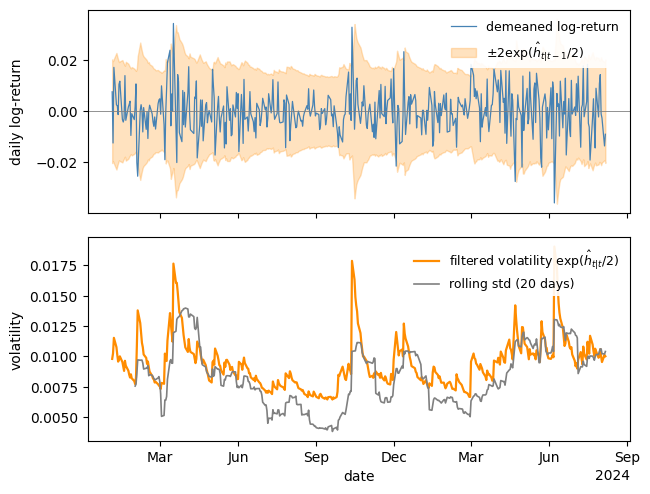
\includegraphics[width=0.8\linewidth]{Figures/sv_filtered_vol.png}
  \caption{The stochastic volatility model on the training returns of the
  gold series. Top: demeaned daily log-returns with the one-step-ahead band
  $\pm 2\exp(\hat{h}_{t\mid t-1}/2)$, which contains $96\%$ of the returns.
  Bottom: filtered volatility $\exp(\hat{h}_{t\mid t}/2)$ with the rolling
  standard deviation of Figure~\ref{fig:vol-clustering} as reference.}\label{fig:sv-filtered-vol}
\end{figure}

The volatility is therefore the one hidden quantity in this chapter that the filter clearly recovers. Whether this also makes it easier to predict is the question of the next section.

\section{Model comparison}\label{sec:model-comparison}

All models so far were built and motivated separately. We now put them on a single, common test, and the outcome is sober, because on daily data none of them beats the simple baselines by much. Table~\ref{tab:model-overview} collects their state space forms in one place. Reading down the rows, the state grows from nothing to a level, then a level with a slope, then the recent returns, and finally a log-variance, and only the last measurement is non-linear.

\begin{table}
\centering
\footnotesize
\renewcommand{\arraystretch}{1.4}
\begin{tabular}{lllll}
\hline
Model & State & Transition & Measurement & Filter \\
\hline
i.i.d. & none & none & $r_t = \mu + \varepsilon_t$ & none \\
Local level & level $x_t$ & random walk \eqref{eq:rw} & $y_t = x_t + \varepsilon_t$ & Kalman \\
Local linear trend & $(\ell_t, b_t)^\top$ & \eqref{eq:llt-state} & $y_t = \ell_t + \varepsilon_t$ & Kalman \\
AR($p$) & last $p$ values & companion form \eqref{eq:ar1-ss} & $y_t = r_t + \varepsilon_t$ & Kalman \\
Stochastic volatility & log-variance $h_t$ & AR(1) \eqref{eq:sv-state} & $z_t = \exp(h_t)\,\xi_t^2$ & extended Kalman \\
\hline
\end{tabular}
\caption{The state space forms of the models in this chapter. The mean models
differ in their state but keep the measurement linear, while the stochastic
volatility model is the only one with a non-linear measurement.}
\label{tab:model-overview}
\end{table}

The forecasts collected on the test part in Section~\ref{sec:framework}, $\hat{y}_{t+1 \mid t} = \mathbb{E}[\,y_{t+1} \mid y_{1:t}\,]$, are ranked by their mean squared prediction error (Definition~\ref{def:mmse}, here applied to the one-step prediction error),
\begin{equation}\label{eq:mse}
  \mathrm{MSE} \;=\; \frac{1}{N}\sum_{t} \bigl(y_{t+1} - \hat{y}_{t+1 \mid t}\bigr)^2 ,
\end{equation}
averaged over the $N$ steps of the test segment. We deliberately score the prediction rather than the filtered residual. The filtered estimate has already seen $y_{t+1}$ and, when the measurement noise is small, can match it almost exactly, whereas the prediction is formed before $y_{t+1}$ arrives and so tests the dynamics the model actually claims.

We run this comparison on the gold series, using daily closing prices. All models are scored on the same quantity, the one-step-ahead log-return, which both scales share as their one-step error (Section~\ref{sec:prices-returns}). The return is scored rather than the price because its error does not depend on the price level and so stays comparable across stretches of the sample and across assets. Table~\ref{tab:mean-mse} reports the one-step-ahead return MSE of each mean model on the test part, together with the naive persistence forecast $\hat{r}_{t+1\mid t}=0$, which predicts no change in the log-price, as a reference point.

\begin{table}
\centering
\begin{tabular}{lr}
\hline
Model & Test MSE $(\times 10^{-5})$ \\
\hline
Persistence $\bigl(\hat{r}_{t+1\mid t}=0\bigr)$ & $9.47$ \\
i.i.d.\ with drift & $9.40$ \\
Local level (Kalman filter) & $9.45$ \\
Local linear trend (Kalman filter) & $9.39$ \\
AR(1) & $9.37$ \\
AR(2) & $9.35$ \\
\hline
\end{tabular}
\caption{One-step-ahead return mean squared error of the mean models on the gold
test segment (daily log-returns, last $20\%$ of the sample). The level models run
on the log-price, whose one-step prediction error equals the return error.}
\label{tab:mean-mse}
\end{table}

The errors are almost the same across all models, and none improves much on the persistence forecast, which is what the efficient market hypothesis leads us to expect. A small and consistent gain does appear once we add structure. Allowing a drift, as in the i.i.d.\ model, and a weak dependence on the recent past, as in the autoregressive models, lowers the error, and AR(2) is marginally the best, about $1.3\%$ below persistence. The fitted autoregressive coefficients are small and negative, which points to a slight tendency of a move to be partly reversed on the following day. On the level of the price there is little to predict, so the question that remains is whether modeling the variance helps.

The stochastic volatility model of Section~\ref{sec:variance-modeling} is not included in Table~\ref{tab:mean-mse}, because it does not forecast the price at all. We score it instead on $\log r_t^2$, the logarithm of the squared demeaned return. Taking logarithms in \eqref{eq:sv-sq} gives $\log r_t^2 = h_t + \log \xi_t^2$, and the noise term $\log \xi_t^2$ has mean approximately $-1.27$~\cite[Section~7.3]{triantafyllopoulos:bayesian_state_space}, so the conditional mean of the target given the state is $h_t - 1.27$. On the test segment the filter runs on $r_t^2$ and its predicted state is converted to the target as $\hat{h}_{t \mid t-1} - 1.27$, scored by \eqref{eq:mse}. The i.i.d.\ model is again the baseline, with the constant prediction $\log \hat{\sigma}^2 - 1.27$, where $\hat{\sigma}^2$ is the return variance of the training segment.

\begin{table}
\centering
\begin{tabular}{lr}
\hline
Model & Test MSE of $\log r_t^2$ \\
\hline
i.i.d.\ (constant variance) & $4.59$ \\
Stochastic volatility (EKF on $r_t^2$) & $4.93$ \\
\hline
\end{tabular}
\caption{One-step-ahead mean squared error of the $\log r_t^2$ prediction on
the gold test segment (daily returns, last $20\%$ of the sample, demeaned with
the training mean).}
\label{tab:sv-mse}
\end{table}

The outcome in Table~\ref{tab:sv-mse} is as sober as the price comparison. The stochastic volatility model does not improve on the constant variance of the i.i.d.\ model. The observation noise alone accounts for almost all of the error in both rows, so both sit essentially at the noise floor, and whatever signal the hidden log-variance carries is small compared to the noise through which it is observed. The fit does find persistent volatility on the training data, with $\varphi = 0.92$, but over the 104 test days this persistence does not translate into better predictions of $\log r_t^2$.  On a short daily gold sample, both the level and the variance of the returns are hard to predict on data the fit has never seen, and simple baselines are difficult to beat. That is the honest result, and it is worth keeping apart from what the chapter did show. The filtering methods of the previous chapters carry over to financial data without modification, and the hidden volatility can be recovered even where recovering it does not improve the forecast. What this means for the value of the exercise, and what one would do differently, is taken up in Chapter~\ref{chap:conclusion}.